\subsection[SGSTM]{Sistemes de gestió de sèries temporals multiresolució (SGSTM)}




\begin{frame}{Multiresolució: exemple}

\begin{center}
\usetikzlibrary{dateplot}    
\begin{tikzpicture}
    \begin{axis}[
        date coordinates in=x,
%        xticklabel={\pgfcalendar{tickcal}{\tick}{\tick}{\pgfcalendarshorthand{m}{.}}},
        xticklabel={\pgfcalendarmonthshortname{\month} \year},
        xticklabel style= {rotate=15,anchor=east},
        xlabel=Time,
        ylabel=Temperature (K),
        ymax = 320,
        clip=false,
        y filter/.code = { \pgfmathparse{(#1>320)*322+(#1<320)*#1}},
        ]
       \addplot[blue] file {dades/matriu0.originalbyday.dat};

%      \node[right] at (axis cs:2011-10-12,330) {\footnotesize(2938)};
       \node (break) at (axis cs:2011-10-02,318)[inner sep=0pt,minimum width=0.75em, minimum height=0.5ex,fill=white] {};
    \draw [fill=red,color=blue] (break.north east) -- (break.north west) (break.south west) -- (break.south east);



  \end{axis}
\end{tikzpicture}



%%% Local Variables:
%%% TeX-master: "../main"
%%% ispell-local-dictionary: "british"
%%% End:

\end{center}

\end{frame}

\begin{frame}{Multiresolució: exemple}

Esquema de multiresolució

\begin{center}
%mrd.afegeix_disc(h5,24,mitjana,zero)
%mrd.afegeix_disc(d2,20,mitjana,zero)
%mrd.afegeix_disc(d15,12,mitjana,zero)
%mrd.afegeix_disc(d50,12,mitjana,zero)
\tiny
\begin{center}
%\begin{multicols}{4} 


    \begin{picture}(14,12)(-7,-6)
    \put(0,-1){\makebox(0,0)[c]{{\color{blue}50 days}}}
      \put(0,0){\circle{10}}
      \put(5,0){\circle{0.8}}
      \put(4.33,2.5){\circle{0.8}}
      \put(2.5,4.33){\circle{0.8}}
      \put(0,5){\circle{0.8}}
      \put(-2.5,4.33){\circle{0.8}}   
      \put(-4.33,2.5){\circle{0.8}}
      \put(-5,0){\circle{0.8}}
      \put(-4.33,-2.5){\circle{0.8}}
      \put(-2.5,-4.33){\circle{0.8}} 
      \put(0,-5){\circle{0.8}}
      \put(2.5,-4.33){\circle{0.8}} 
      \put(4.33,-2.5){\circle{0.8}}
      \put(0,0){\vector(0,1){5}}
      \put(0,0){\oval(5,5)[t]}
      \put(-2.5,0){\makebox(0,0)[c]{$\vee$}}
    \end{picture}
%
    \begin{picture}(14,12)(-7,-6)
    \put(0,-1){\makebox(0,0)[c]{{\color{brown}15 days}}}
      \put(0,0){\circle{10}}
      \put(5,0){\circle{0.8}}
      \put(4.33,2.5){\circle{0.8}}
      \put(2.5,4.33){\circle{0.8}}
      \put(0,5){\circle{0.8}}
      \put(-2.5,4.33){\circle{0.8}}   
      \put(-4.33,2.5){\circle{0.8}}
      \put(-5,0){\circle{0.8}}
      \put(-4.33,-2.5){\circle{0.8}}
      \put(-2.5,-4.33){\circle{0.8}} 
      \put(0,-5){\circle{0.8}}
      \put(2.5,-4.33){\circle{0.8}} 
      \put(4.33,-2.5){\circle{0.8}}
      \put(0,0){\vector(0,1){5}}
      \put(0,0){\oval(5,5)[t]}
      \put(-2.5,0){\makebox(0,0)[c]{$\vee$}}
    \end{picture}
%
    \begin{picture}(14,12)(-7,-6)
    \put(0,-1){\makebox(0,0)[c]{{\color{red}2 days}}}
      \put(0,0){\circle{10}}
      %\put(5,0){\circle{0.8}}
      \put(4.82,1.29){\circle{0.8}}
      \put(4.33,2.5){\circle{0.8}}
     \put(3.5,3.5){\circle{0.8}}
      \put(2.5,4.33){\circle{0.8}}
      \put(1.29,4.82){\circle{0.8}}
      %\put(0,5){\circle{0.8}}
      \put(-1.29,4.82){\circle{0.8}}
      \put(-2.5,4.33){\circle{0.8}}
       \put(-3.5,3.5){\circle{0.8}} 
      \put(-4.33,2.5){\circle{0.8}}
    \put(-4.82,1.29){\circle{0.8}}
      %\put(-5,0){\circle{0.8}}
    \put(-4.82,-1.29){\circle{0.8}}
      \put(-4.33,-2.5){\circle{0.8}}
      \put(-3.5,-3.5){\circle{0.8}} 
      \put(-2.5,-4.33){\circle{0.8 } } 
      \put(-1.29,-4.82){\circle{0.8 }}
      % \put(0,-5){\circle{0.8 }}
     \put(1.29,-4.82){\circle{0.8 }}
      \put(2.5,-4.33){\circle{0.8}}
      \put(3.5,-3.5){\circle{0.8}} 
      \put(4.33,-2.5){\circle{0.8}}
  \put(4.82,-1.29){\circle{0.8}}
      \put(0,0){\vector(0,1){5}}
      \put(0,0){\oval(5,5)[t]}
      \put(-2.5,0){\makebox(0,0)[c]{$\vee$}}
    \end{picture}
%
    \begin{picture}(14,12)(-7,-6)
    \put(0,-1){\makebox(0,0)[c]{{\color{cyan}5 hours}}}
      \put(0,0){\circle{10}}
      \put(5,0){\circle{0.8}}
      \put(4.82,1.29){\circle{0.8}}
      \put(4.33,2.5){\circle{0.8}}
     \put(3.5,3.5){\circle{0.8}}
      \put(2.5,4.33){\circle{0.8}}
      \put(1.29,4.82){\circle{0.8}}
      \put(0,5){\circle{0.8}}
      \put(-1.29,4.82){\circle{0.8}}
      \put(-2.5,4.33){\circle{0.8}}
       \put(-3.5,3.5){\circle{0.8}} 
      \put(-4.33,2.5){\circle{0.8}}
    \put(-4.82,1.29){\circle{0.8}}
      \put(-5,0){\circle{0.8}}
    \put(-4.82,-1.29){\circle{0.8}}
      \put(-4.33,-2.5){\circle{0.8}}
      \put(-3.5,-3.5){\circle{0.8}} 
      \put(-2.5,-4.33){\circle{0.8 } } 
      \put(-1.29,-4.82){\circle{0.8 }}
\put(0,-5){\circle{0.8 }}
     \put(1.29,-4.82){\circle{0.8 }}
      \put(2.5,-4.33){\circle{0.8}}
      \put(3.5,-3.5){\circle{0.8}} 
      \put(4.33,-2.5){\circle{0.8}}
  \put(4.82,-1.29){\circle{0.8}}
      \put(0,0){\vector(0,1){5}}
      \put(0,0){\oval(5,5)[t]}
      \put(-2.5,0){\makebox(0,0)[c]{$\vee$}}
    \end{picture}


%\end{multicols}

\vspace{-10pt}

\setlength{\unitlength}{900sp}
\begin{picture}(14460,5066)(7322,-7148)
\thinlines
{\color[rgb]{0,0,0}\put(7300,-6271){\line( 0,-1){386}}
}%
{\color[rgb]{0,0,0}\put(7782,-6271){\line( 0,-1){386}}
}%
{\color[rgb]{0,0,0}\put(8263,-6271){\line( 0,-1){386}}
}%
{\color[rgb]{0,0,0}\put(8745,-6271){\line( 0,-1){386}}
}%
{\color[rgb]{0,0,0}\put(9227,-6271){\line( 0,-1){386}}
}%
{\color[rgb]{0,0,0}\put(9709,-6271){\line( 0,-1){386}}
}%
{\color[rgb]{0,0,0}\put(10191,-6271){\line( 0,-1){386}}
}%
{\color[rgb]{0,0,0}\put(10673,-6271){\line( 0,-1){386}}
}%
{\color[rgb]{0,0,0}\put(11155,-6271){\line( 0,-1){386}}
}%
{\color[rgb]{0,0,0}\put(11637,-6271){\line( 0,-1){386}}
}%
{\color[rgb]{0,0,0}\put(12119,-6271){\line( 0,-1){386}}
}%
{\color[rgb]{0,0,0}\put(12600,-6271){\line( 0,-1){386}}
}%
{\color[rgb]{0,0,0}\put(13082,-6271){\line( 0,-1){386}}
}%
{\color[rgb]{0,0,0}\put(13564,-6271){\line( 0,-1){386}}
}%
{\color[rgb]{0,0,0}\put(14046,-6271){\line( 0,-1){386}}
}%
{\color[rgb]{0,0,0}\put(14528,-6271){\line( 0,-1){386}}
}%
{\color[rgb]{0,0,0}\put(15010,-6271){\line( 0,-1){386}}
}%
{\color[rgb]{0,0,0}\put(15492,-6271){\line( 0,-1){386}}
}%
{\color[rgb]{0,0,0}\put(15974,-6271){\line( 0,-1){386}}
}%
{\color[rgb]{0,0,0}\put(16456,-6271){\line( 0,-1){386}}
}%
{\color[rgb]{0,0,0}\put(16938,-6271){\line( 0,-1){386}}
}%
{\color[rgb]{0,0,0}\put(17419,-6271){\line( 0,-1){386}}
}%
{\color[rgb]{0,0,0}\put(17901,-6271){\line( 0,-1){386}}
}%
{\color[rgb]{0,0,0}\put(18383,-6271){\line( 0,-1){386}}
}%
{\color[rgb]{0,0,0}\put(18865,-6271){\line( 0,-1){386}}
}%
{\color[rgb]{0,0,0}\put(19347,-6271){\line( 0,-1){386}}
}%
{\color[rgb]{0,0,0}\put(19829,-6271){\line( 0,-1){386}}
}%
{\color[rgb]{0,0,0}\put(20311,-6271){\line( 0,-1){386}}
}%
{\color[rgb]{0,0,0}\put(20793,-6271){\line( 0,-1){386}}
}%
{\color[rgb]{0,0,0}\put(21275,-6271){\line( 0,-1){386}}
}%
{\color[rgb]{0,0,0}\put(7300,-6271){\line( 0,-1){1157}}
}%
{\color[rgb]{0,0,0}\put(9709,-6271){\line( 0,-1){1157}}
}%
{\color[rgb]{0,0,0}\put(12119,-6271){\line( 0,-1){1157}}
}%
{\color[rgb]{0,0,0}\put(14528,-6271){\line( 0,-1){1157}}
}%
{\color[rgb]{0,0,0}\put(16938,-6271){\line( 0,-1){1157}}
}%
{\color[rgb]{0,0,0}\put(19347,-6271){\line( 0,-1){1157}}
}%
{\color[rgb]{0,0,0}\put(21756,-6271){\line( 0,-1){1157}}
}%
{\color[rgb]{0,0,0}\put(7300,-6271){\line( 1, 0){14456}}
}%

\put(7322,-6271){\line( 0,1){3000}}
\put(21756,-7783){\makebox(0,0)[b]{now}}%
\put(7322,-7783){\makebox(0,0)[b]{600 days back}}%

\color{blue}
\put(21782,-5928){\line( -1,0){14460}}
\put(21782,-5928){\line( 0,1){779}}
\put(21782,-5149){\line( -1,0){14460}}
\put(7322,-5928){\line( 0,1){779}}
\put(14530,-5450){\makebox(0,0)[c]{600 days}}

\color{brown}
\put(21782,-5149){\line( 0,1){779}}
\put(21782,-4370){\line( -1,0){4438}}
\put(17344,-5149){\line( 0,1){779}}
\put(19563,-4800){\makebox(0,0)[c]{180 days}}

\color{red}
\put(21782,-4370){\line( 0,1){779}}
\put(21782,-3591){\line( -1,0){964}}
\put(20818,-4370){\line( 0,1){779}}
\put(21300,-3950){\makebox(0,0)[c]{40d}}

\color{cyan}
\put(21782,-3591){\line( 0,1){779}}
\put(21782,-2812){\line( -1,0){120}}
\put(21661,-3591){\line( 0,1){779}}
\put(21300,-3201){\makebox(0,0)[c]{5d}}
\end{picture}%


\normalsize

\end{center}
\end{center}

\end{frame}

\begin{frame}{Multiresolució: exemple}


\begin{center}

  \begin{tikzpicture}[scale=0.6, every node/.style={transform shape}]
    \begin{axis}[
        multiresoluciodate,
        title={$R_1$: 5h $|24|$},
        xticklabel={\day--\hour:\minute},
        clip=false,
        ]
       \addplot[const plot mark right, blue] table[col sep=comma] {imatges/exemple/dades-matriu0/R18000mean_zohe.csv};
     \node[left] at (axis cs:2011-10-19,274) {\footnotesize oct.~2011};
  \end{axis}
\end{tikzpicture}
%
  \begin{tikzpicture}[scale=0.6, every node/.style={transform shape}]
    \begin{axis}[
        multiresoluciodate,
        title={$R_2$: 2d $|20|$},
        xticklabel={\day~\pgfcalendarmonthshortname{\month}},
        clip=false,
        ]
       \addplot[const plot mark right, blue] table[col sep=comma] {imatges/exemple/dades-matriu0/R172800mean_zohe.csv};
     \node[left] at (axis cs:2011-10-21,279) {\footnotesize 2011};
  \end{axis}
\end{tikzpicture}
%
  \begin{tikzpicture}[scale=0.6, every node/.style={transform shape}]
    \begin{axis}[
        multiresoluciodate,
        title={$R_3$: 15d $|12|$},
        xticklabel={\day~\pgfcalendarmonthshortname{\month}},
        y filter/.code = { \pgfmathparse{(#1>320)*330+(#1<320)*#1}},
        ymax = 320,
        clip=false,
        ]

       \addplot[const plot mark right, blue] table[col sep=comma] {imatges/exemple/dades-matriu0/R1296000mean_zohe.csv};

      \addplot[const plot mark right, orange] table[col sep=comma] {imatges/exemple/dades-matriu0/R1296000maximum_zohe.csv};

      \node[right] at (axis cs:2011-10-07,330) {\footnotesize(2938)};
       \node (break) at (axis cs:2011-09-23,325)[inner sep=0pt,minimum width=0.75em, minimum height=0.5ex,fill=white] {};
    \draw [fill=red,color=orange] (break.north east) -- (break.north west) (break.south west) -- (break.south east);

     \node[left] at (axis cs:2011-10-27,273) {\footnotesize 2011};

  \end{axis}
\end{tikzpicture}
%
\begin{tikzpicture}[scale=0.6, every node/.style={transform shape}]
    \begin{axis}[
        multiresoluciodate,
        xticklabel={\pgfcalendarmonthshortname{\month}~\year},
        title={$R_4$: 50d $|12|$},
        xlabel={Temps (UTC)},
%        ylabel={Temperatura (K)},
        ymax = 320,
        clip=false,
%v1.6     restrict y to domain=0:320,
        y filter/.code = { \pgfmathparse{(#1>320)*330+(#1<320)*#1}},
        ]

       \addplot[const plot mark right, blue] table[col sep=comma] {imatges/exemple/dades-matriu0/R4320000mean_zohe.csv};
       \addlegendentry{mitjana};

       \addplot[const plot mark right, orange] table[col sep=comma] {imatges/exemple/dades-matriu0/R4320000maximum_zohe.csv};
       \addlegendentry{màxim};

       \node[right] at (axis cs:2011-10-12,330) {\footnotesize(2938)};
       \node (break) at (axis cs:2011-08-24,325)[inner sep=0pt,minimum width=0.75em, minimum height=0.5ex,fill=white] {};
    \draw [fill=red,color=orange] (break.north east) -- (break.north west) (break.south west) -- (break.south east);

  \end{axis}
\end{tikzpicture}




%%% Local Variables:
%%% TeX-master: "../../main"
%%% End:

\end{center}

\end{frame}

\begin{frame}{Multiresolució: exemple}

Consulta de les sèries temporals emmagatzemades

\begin{center}
\usetikzlibrary{dateplot}  
%\usetikzlibrary{pgfplots.groupplots}

\pgfplotsset{
   petit/.style={
        ylabel=Temperature (K),
%        width=\textwidth,
%        height=3.5cm,
        legend style={font=\footnotesize},
        tick label style={font=\footnotesize},
        label style={font=\tiny},
        title style={font=\small,below, anchor=north,fill=white},
        xticklabel style= {rotate=15,anchor=east},
%        every axis title shift=0pt,
%        max space between ticks=15,
        every mark/.append style={mark size=6},
        major tick length=0.1cm,
        minor tick length=0.066cm,
        very thin,
        every axis legend/.append style={
          at={(1,0.02)},
          anchor=south east,
          draw = none},
        legend columns = 4,
    }
}

\begin{tikzpicture}
    \begin{axis}[
        petit,
        date coordinates in=x,
        xticklabel={\pgfcalendarmonthshortname{\month} \year},
        xlabel=Time (UTC),
%        unbounded coords=jump, %v>1.4
%        unbounded coords=discard, %v>1.4
        ymax = 320,
        clip=false,
%v1.6     restrict y to domain=0:320,
        y filter/.code = { \pgfmathparse{(#1>320)*330+(#1<320)*#1}},
        ]

       \addplot[black!15] file {dades/matriu0.originalbyday.dat};
       \addlegendentry{original};

       \addplot[blue] table[col sep=comma] {dades/mrdb-matriu0/union1.csv};
       \addlegendentry{mean};

       \addplot[orange] table[col sep=comma] {dades/mrdb-matriu0/union0.csv};
       \addlegendentry{max};

%       \node[right] at (axis cs:2011-10-12,330) {\mbox{(2938)}};
       \node (break) at (axis cs:2011-09-25,325)[inner sep=0pt,minimum width=0.9em, minimum height=0.4ex,fill=white] {};
    \draw [fill=red,color=orange] (break.north east) -- (break.north west) (break.south west) -- (break.south east);


  \end{axis}
\end{tikzpicture}
%http://tex.stackexchange.com/questions/46422/axis-break-in-pgfplots

%http://tex.stackexchange.com/questions/52409/insert-a-separate-mark-inside-a-pgfplots-graph



%%% Local Variables:
%%% TeX-master: "../main"
%%% ispell-local-dictionary: "british"
%%% End:

\end{center}

\end{frame}




\begin{frame}{SGSTM - Estructura}
\begin{columns}
  
  \column{4cm}
  Conceptes:
  \begin{itemize}

  \item Buffer
  \item Disc
  \item Subsèrie resolució
  \item Sèrie temporal multiresolució
  \item Esquema de multiresolució: Conjunt de resolucions (pas, temps d'inici, cardinal, funció d'agregació)

  \end{itemize}

  \column{6cm}


\begin{tikzpicture}[scale=0.7, every node/.style={transform shape}]
 \tikzset{
        myarrow/.style={->, >=latex',  thick},
      }
      

  \node[rectangle,draw,minimum height=6cm,minimum width=9cm] (m) {};
  \draw[shift=( m.south west)]   
  node[above right] {sèrie temporal multiresolució};


  %discmig
  \node (m.center) (discr1) {...};

  %discr
  
  \node[ellipse,draw,minimum height=3.5cm,minimum width=2.5cm,alias=discr0] [left=of discr1] {};
  \node[above=0cm of discr0.north] {$R_0$};
  \node[below=0cm of discr0] {subsèrie resolució};

  \node[cylinder, draw, shape border rotate=90, aspect=0.25,alias=buffer0] [below=3mm of discr0.north] {buffer};
  \node[circle, draw,alias=disc0]  [above=3mm of discr0.south] {disc} ;
  \draw [->] (disc0.center)++(.4:.4cm) arc(0:180:.4cm);
  \draw[myarrow] (buffer0.bottom) -- (disc0.north);


  %discrd

  \node[ellipse,draw,minimum height=3.5cm,minimum width=2.5cm,alias=discrd] [right=of discr1] {};
  \node[above=0cm of discrd] {$R_d$};
  \node[below=0cm of discrd] {subsèrie resolució};

  \node[cylinder, draw, shape border rotate=90, aspect=0.25,alias=bufferd] [below=3mm of discrd.north] {buffer};
  \node[circle, draw,alias=discd]  [above=3mm of discrd.south] {disc} ;
  \draw [->] (discd.center)++(.4:.4cm) arc(0:180:.4cm);
  \draw[myarrow] (bufferd.bottom) -- (discd.north);



  %mesura 
  \node[above=1cm of m.north] (m0) {};

  \draw[myarrow] (m0) -- (m.north) 
  node[right,midway] {mesura};

  \draw[myarrow] (m.north) -- (buffer0);
  \draw[myarrow] (m.north) -- (bufferd);
  \draw[myarrow] (m.north) -- (discr1);

\end{tikzpicture}


\end{columns}
\end{frame}




\begin{frame}{SGSTM - Operacions}

  \begin{itemize}
  \item Estructurals: 
    \begin{itemize}
    \item afegir mesura als buffers 
    \item consolidar les resolucions
    \end{itemize}

  \item Manipulació de l'esquema

  \item Consultes
    \begin{itemize}
    \item extracció de subsèries
    \item sèrie temporal total
    \end{itemize}

  \end{itemize}


\end{frame}


\begin{frame}{SGSTM - Funcions d'agregació d'atributs}

\begin{centering}

 mesura = funció(sèrie temporal, interval de consolidació)


   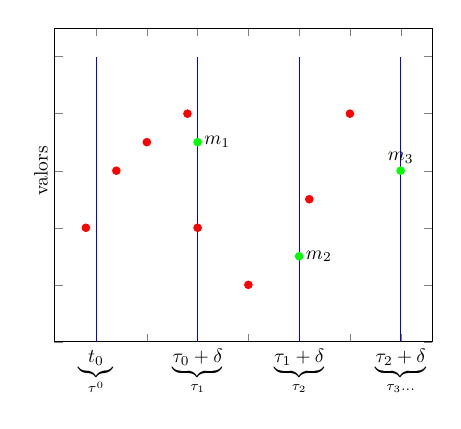
\begin{tikzpicture}[scale=0.7, every node/.style={transform shape}]
    \begin{axis}[
        ymin = 0,
        yticklabels= {,,,,valors},
        y tick label style = {rotate=90,anchor=south},
        xticklabels={,,$\underbrace{t_0 \vphantom{\delta}}_{\tau^0}$,,$\underbrace{\tau_0+\delta}_{\tau_1}$,,$\underbrace{\tau_1+\delta}_{\tau_2}$,,$\underbrace{\tau_2+\delta}_{\tau_3 \ldots}$},
        ]
 
    \addplot[ycomb,blue] coordinates {
        (20,10)
        (30,10)
        (40,10)
        (50,10)
    }; 

    \addplot[red,only marks, mark = *] coordinates {
        (19,4)
        (22,6)
        (25,7)
        (29,8)
        (30,4)
        (35,2)
        (41,5)
        (45,8)
    };

          \addplot[only marks,mark=*,green] coordinates {
            (30,7)
            (40,3)
            (50,6)
          };

          \node[right] at (axis cs:30,7) {$m_1$};
          \node[right] at (axis cs:40,3) {$m_2$};
          \node[above] at (axis cs:50,6) {$m_3$};
    \end{axis}
  \end{tikzpicture}

\end{centering}

\begin{itemize}
  \item agregació amb representació
  \item tractament i validació de dades
  \end{itemize}


\end{frame}


%%% Local Variables: 
%%% mode: latex
%%% TeX-master: "defensa"
%%% End: 
%  LocalWords:  multiresolució
